\documentclass{gescons}

\genre {Entrevista}
\author{Ana Luiza Rezende e Mabel Teles (Org.)}
\title{Epicentrismo Consciencial: Casuísticas Recinológicas}

\begin{document}
    \makeentrevistatitle
    \coverart{back/Mabel_Teles_Ana_Luiza_Rezende}

    \begin{multicols}{2}

%\noindent\includegraphics[width=9cm, height=10cm]{example-image} 

\begin{center}
    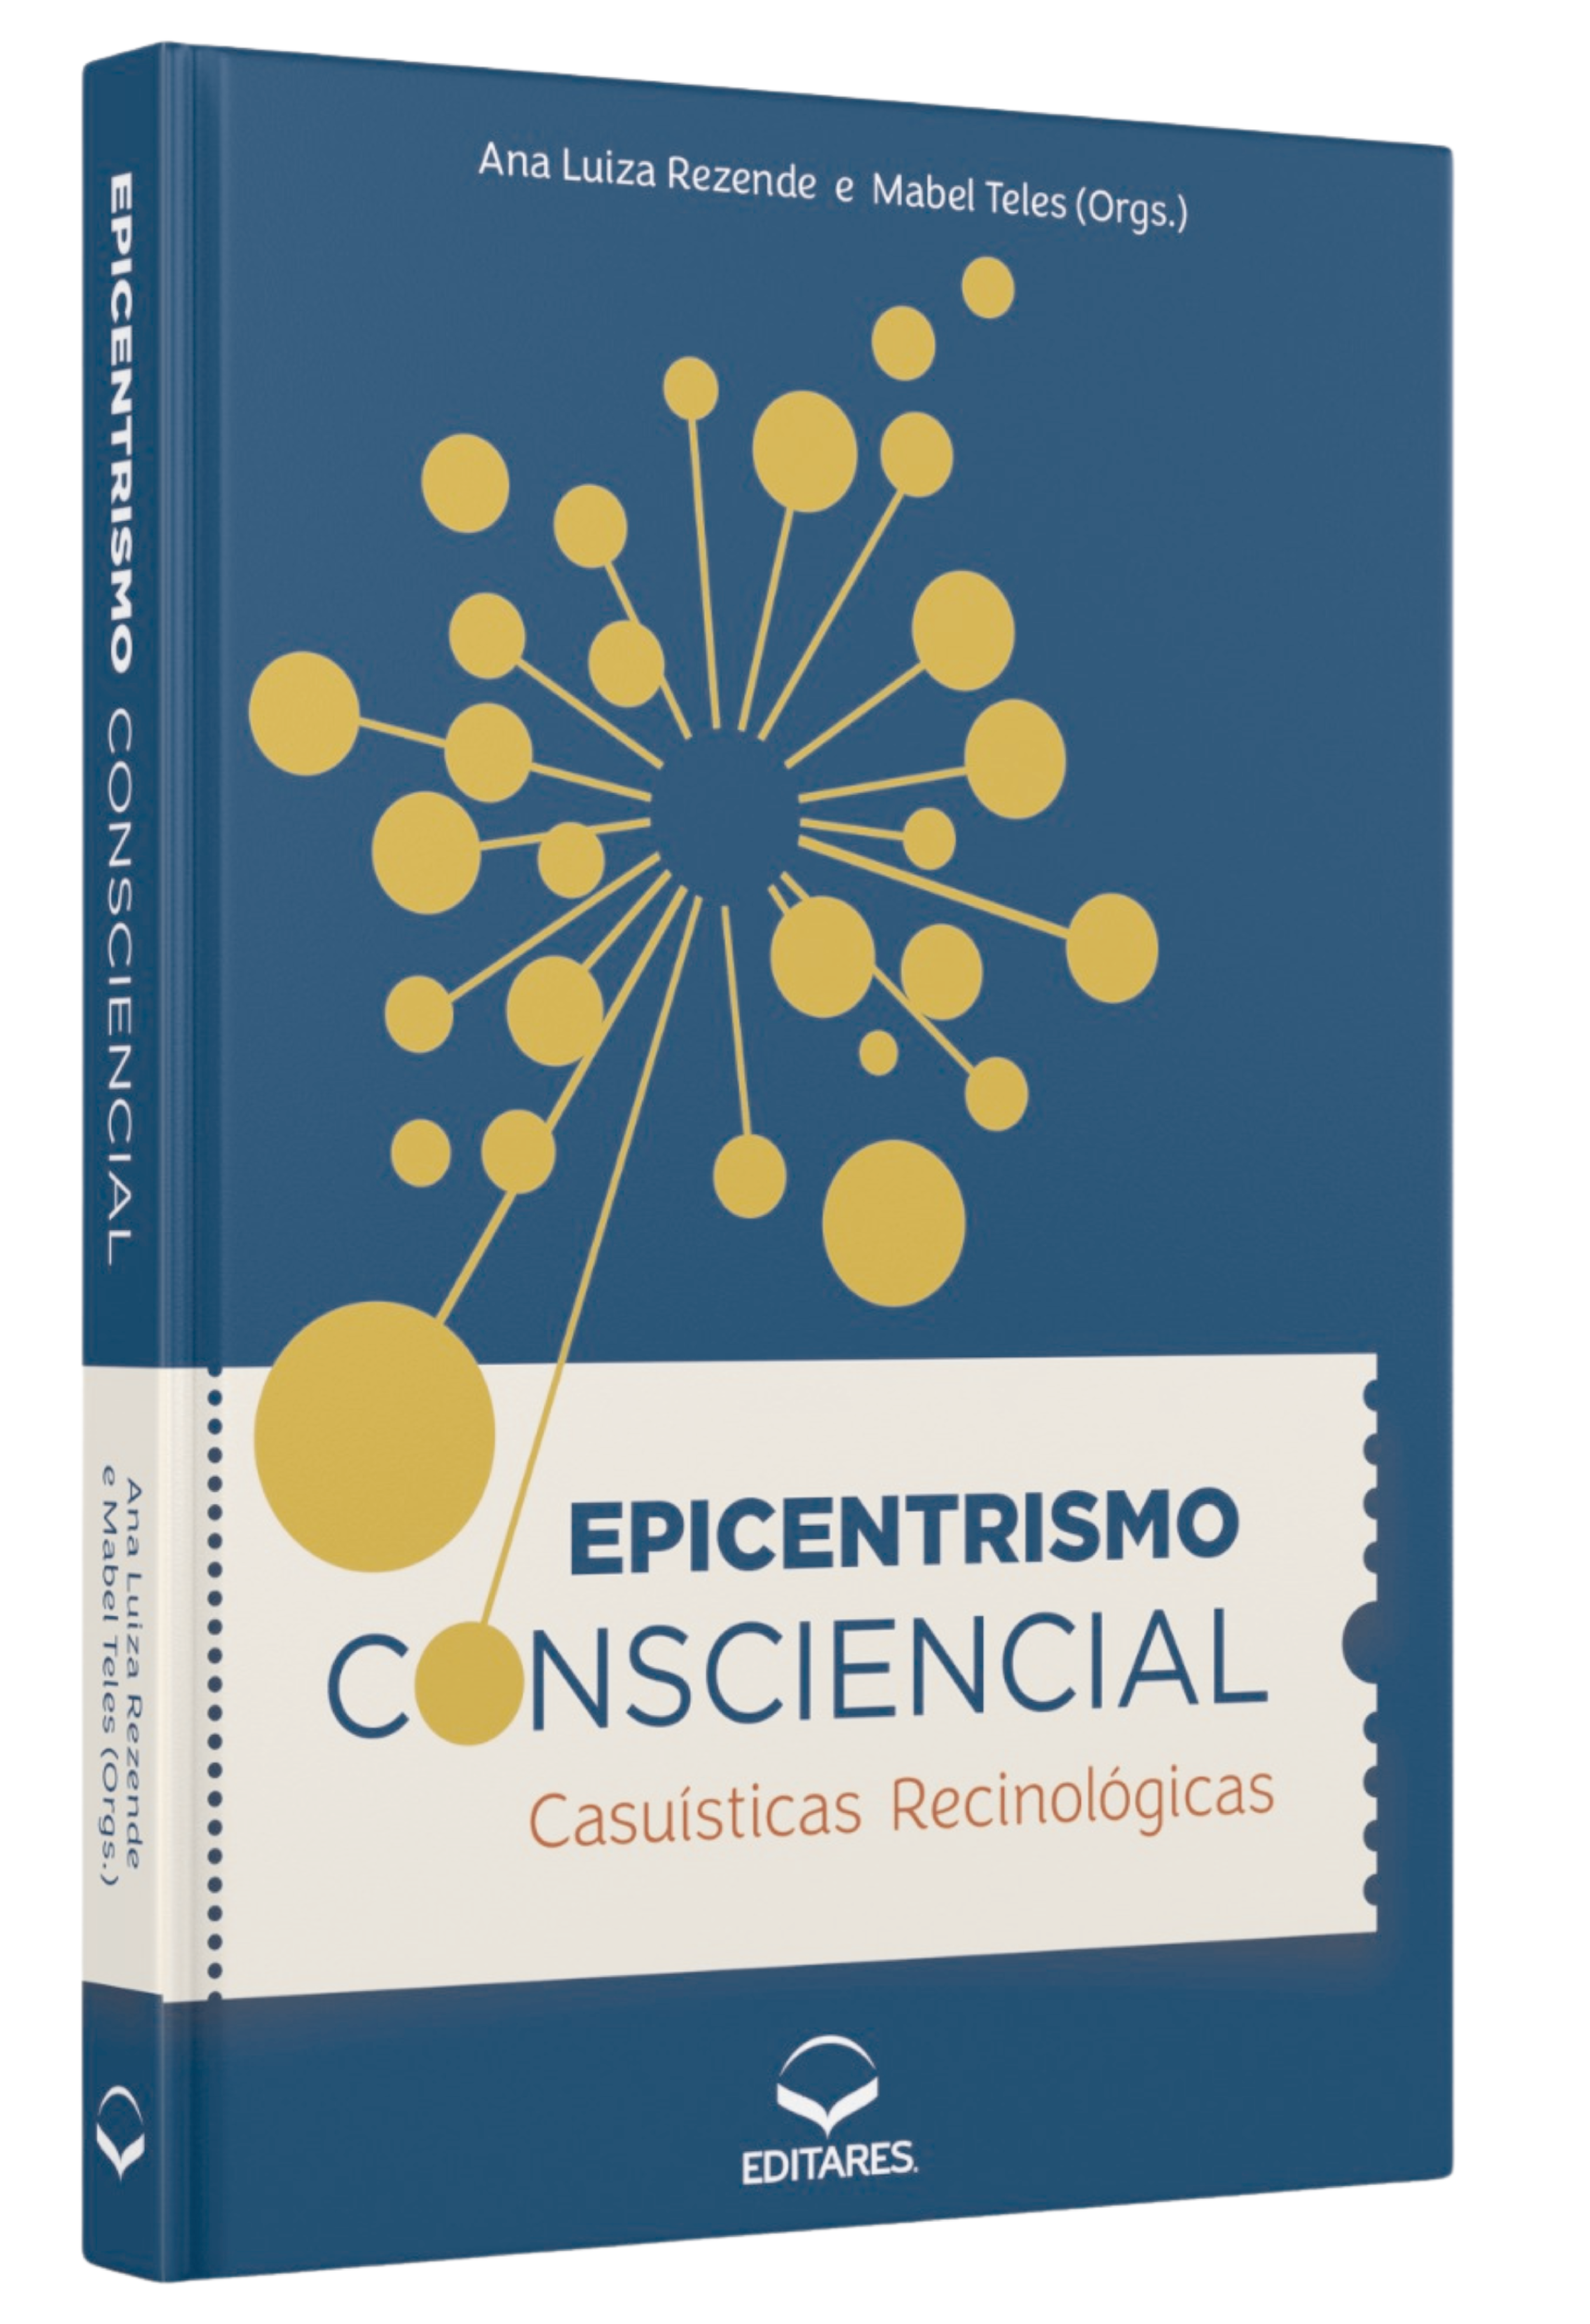
\includegraphics[width=8cm]{articles/entrevista/mockups/Mabel-e-Ana-Luiza.png}
\end{center}

\textbf{Qual foi a motivação para a escrita da obra? Por que a definição deste tema para publicação de um livro?}


O livro \textit{Epicentrismo Consciencial – Casuísticas Recinológicas} surgiu a partir de uma sugestão do Prof. Waldo Vieira (1932-2015), em reunião do \textit{Conselho de Epicons} (CE), realizada no \textit{Hotel Interludium,} Foz do Iguaçu, em 2015. Na ocasião, ele propôs um levantamento das recins e recéxis positivas e exemplaristas já implementadas pelos integrantes do CE. A obra é fruto dessa proposta e busca responder à questão levantada no encontro: \textit{quais atos vêm qualificando o epicentrismo de cada integrante do CE até agora? }

\textbf{2. Quais foram as principais percepções, intra e extrafísicas, durante a pesquisa e a escrita da obra? E posterior ao lançamento?}

A obra, de cunha biográfico, possibilitou o resgate de vivências significativas que contribuíram para o desenvolvimento do epicentrismo de cada autor. O registro de acertos e reciclagens permitiu a identificação de padrões evolutivos pessoais, fortalecendo a responsabilidade perante a grupalidade e a interassistência. A publicação tem incentivado pesquisadores conscienciológicos a aprofundarem as próprias reciclagens, visando a qualificação do autepicentrismo e o aprimoramento da assistência multidimensional.  

\begin{pullquote}
``A obra, de cunha biográfico, possibilitou o resgate de vivências significativas que contribuíram para o desenvolvimento do epicentrismo de cada autor.''
\end{pullquote}


\textbf{3. Qual o maior aprendizado com a escrita desta obra?}

A escrita da obra permitiu o aprofundamento da autopesquisas, além de ter demonstrado a relevância da grupalidade na evolução pessoal, destacando como as interações, os desafios e os aprendizados coletivos fortalecem o epicentrismo de cada um. 


\textbf{4. O que poderiam dizer como incentivo para que mais pesquisadores invistam na publicação de obras conscienciológicas?}

Publicar obras conscienciológicas é uma forma de aprofundar a autopesquisa, consolidar a cognição evolutiva e expandir a interassistência. O registro das experiências cria um legado evolutivo, beneficiando tanto o autor quanto os leitores. Além disso, fortalece a rede de pesquisadores e contribui para a ampliação do paradigma consciencial, estimulando novas reflexões e descobertas.


\begin{pullquote}
``Publicar obras conscienciológicas é uma forma de aprofundar a autopesquisa, consolidar a cognição evolutiva e expandir a interassistência.''
\end{pullquote}




    \end{multicols}
\end{document}















